% Options for packages loaded elsewhere
\PassOptionsToPackage{unicode}{hyperref}
\PassOptionsToPackage{hyphens}{url}
%
\documentclass[
  ignorenonframetext,
  aspectratio=169,
]{beamer}
\usepackage{pgfpages}
\setbeamertemplate{caption}[numbered]
\setbeamertemplate{caption label separator}{: }
\setbeamercolor{caption name}{fg=normal text.fg}
\beamertemplatenavigationsymbolshorizontal
% Prevent slide breaks in the middle of a paragraph
\widowpenalties 1 10000
\raggedbottom
\setbeamertemplate{part page}{
  \centering
  \begin{beamercolorbox}[sep=16pt,center]{part title}
    \usebeamerfont{part title}\insertpart\par
  \end{beamercolorbox}
}
\setbeamertemplate{section page}{
  \centering
  \begin{beamercolorbox}[sep=12pt,center]{part title}
    \usebeamerfont{section title}\insertsection\par
  \end{beamercolorbox}
}
\setbeamertemplate{subsection page}{
  \centering
  \begin{beamercolorbox}[sep=8pt,center]{part title}
    \usebeamerfont{subsection title}\insertsubsection\par
  \end{beamercolorbox}
}
\AtBeginPart{
  \frame{\partpage}
}
\AtBeginSection{
  \ifbibliography
  \else
    \frame{\sectionpage}
  \fi
}
\AtBeginSubsection{
  \frame{\subsectionpage}
}

\usepackage{amsmath,amssymb}
\usepackage{iftex}
\ifPDFTeX
  \usepackage[T1]{fontenc}
  \usepackage[utf8]{inputenc}
  \usepackage{textcomp} % provide euro and other symbols
\else % if luatex or xetex
  \usepackage{unicode-math}
  \defaultfontfeatures{Scale=MatchLowercase}
  \defaultfontfeatures[\rmfamily]{Ligatures=TeX,Scale=1}
\fi
\usepackage{lmodern}
\usetheme[]{Montpellier}
\usecolortheme{seagull}
\ifPDFTeX\else  
    % xetex/luatex font selection
\fi
% Use upquote if available, for straight quotes in verbatim environments
\IfFileExists{upquote.sty}{\usepackage{upquote}}{}
\IfFileExists{microtype.sty}{% use microtype if available
  \usepackage[]{microtype}
  \UseMicrotypeSet[protrusion]{basicmath} % disable protrusion for tt fonts
}{}
\usepackage{xcolor}
\newif\ifbibliography
\setlength{\emergencystretch}{3em} % prevent overfull lines
\setcounter{secnumdepth}{5}

\usepackage{color}
\usepackage{fancyvrb}
\newcommand{\VerbBar}{|}
\newcommand{\VERB}{\Verb[commandchars=\\\{\}]}
\DefineVerbatimEnvironment{Highlighting}{Verbatim}{commandchars=\\\{\}}
% Add ',fontsize=\small' for more characters per line
\usepackage{framed}
\definecolor{shadecolor}{RGB}{241,243,245}
\newenvironment{Shaded}{\begin{snugshade}}{\end{snugshade}}
\newcommand{\AlertTok}[1]{\textcolor[rgb]{0.68,0.00,0.00}{#1}}
\newcommand{\AnnotationTok}[1]{\textcolor[rgb]{0.37,0.37,0.37}{#1}}
\newcommand{\AttributeTok}[1]{\textcolor[rgb]{0.40,0.45,0.13}{#1}}
\newcommand{\BaseNTok}[1]{\textcolor[rgb]{0.68,0.00,0.00}{#1}}
\newcommand{\BuiltInTok}[1]{\textcolor[rgb]{0.00,0.23,0.31}{#1}}
\newcommand{\CharTok}[1]{\textcolor[rgb]{0.13,0.47,0.30}{#1}}
\newcommand{\CommentTok}[1]{\textcolor[rgb]{0.37,0.37,0.37}{#1}}
\newcommand{\CommentVarTok}[1]{\textcolor[rgb]{0.37,0.37,0.37}{\textit{#1}}}
\newcommand{\ConstantTok}[1]{\textcolor[rgb]{0.56,0.35,0.01}{#1}}
\newcommand{\ControlFlowTok}[1]{\textcolor[rgb]{0.00,0.23,0.31}{#1}}
\newcommand{\DataTypeTok}[1]{\textcolor[rgb]{0.68,0.00,0.00}{#1}}
\newcommand{\DecValTok}[1]{\textcolor[rgb]{0.68,0.00,0.00}{#1}}
\newcommand{\DocumentationTok}[1]{\textcolor[rgb]{0.37,0.37,0.37}{\textit{#1}}}
\newcommand{\ErrorTok}[1]{\textcolor[rgb]{0.68,0.00,0.00}{#1}}
\newcommand{\ExtensionTok}[1]{\textcolor[rgb]{0.00,0.23,0.31}{#1}}
\newcommand{\FloatTok}[1]{\textcolor[rgb]{0.68,0.00,0.00}{#1}}
\newcommand{\FunctionTok}[1]{\textcolor[rgb]{0.28,0.35,0.67}{#1}}
\newcommand{\ImportTok}[1]{\textcolor[rgb]{0.00,0.46,0.62}{#1}}
\newcommand{\InformationTok}[1]{\textcolor[rgb]{0.37,0.37,0.37}{#1}}
\newcommand{\KeywordTok}[1]{\textcolor[rgb]{0.00,0.23,0.31}{#1}}
\newcommand{\NormalTok}[1]{\textcolor[rgb]{0.00,0.23,0.31}{#1}}
\newcommand{\OperatorTok}[1]{\textcolor[rgb]{0.37,0.37,0.37}{#1}}
\newcommand{\OtherTok}[1]{\textcolor[rgb]{0.00,0.23,0.31}{#1}}
\newcommand{\PreprocessorTok}[1]{\textcolor[rgb]{0.68,0.00,0.00}{#1}}
\newcommand{\RegionMarkerTok}[1]{\textcolor[rgb]{0.00,0.23,0.31}{#1}}
\newcommand{\SpecialCharTok}[1]{\textcolor[rgb]{0.37,0.37,0.37}{#1}}
\newcommand{\SpecialStringTok}[1]{\textcolor[rgb]{0.13,0.47,0.30}{#1}}
\newcommand{\StringTok}[1]{\textcolor[rgb]{0.13,0.47,0.30}{#1}}
\newcommand{\VariableTok}[1]{\textcolor[rgb]{0.07,0.07,0.07}{#1}}
\newcommand{\VerbatimStringTok}[1]{\textcolor[rgb]{0.13,0.47,0.30}{#1}}
\newcommand{\WarningTok}[1]{\textcolor[rgb]{0.37,0.37,0.37}{\textit{#1}}}

\providecommand{\tightlist}{%
  \setlength{\itemsep}{0pt}\setlength{\parskip}{0pt}}\usepackage{longtable,booktabs,array}
\usepackage{calc} % for calculating minipage widths
\usepackage{caption}
% Make caption package work with longtable
\makeatletter
\def\fnum@table{\tablename~\thetable}
\makeatother
\usepackage{graphicx}
\makeatletter
\def\maxwidth{\ifdim\Gin@nat@width>\linewidth\linewidth\else\Gin@nat@width\fi}
\def\maxheight{\ifdim\Gin@nat@height>\textheight\textheight\else\Gin@nat@height\fi}
\makeatother
% Scale images if necessary, so that they will not overflow the page
% margins by default, and it is still possible to overwrite the defaults
% using explicit options in \includegraphics[width, height, ...]{}
\setkeys{Gin}{width=\maxwidth,height=\maxheight,keepaspectratio}
% Set default figure placement to htbp
\makeatletter
\def\fps@figure{htbp}
\makeatother
% definitions for citeproc citations
\NewDocumentCommand\citeproctext{}{}
\NewDocumentCommand\citeproc{mm}{%
  \begingroup\def\citeproctext{#2}\cite{#1}\endgroup}
\makeatletter
 % allow citations to break across lines
 \let\@cite@ofmt\@firstofone
 % avoid brackets around text for \cite:
 \def\@biblabel#1{}
 \def\@cite#1#2{{#1\if@tempswa , #2\fi}}
\makeatother
\newlength{\cslhangindent}
\setlength{\cslhangindent}{1.5em}
\newlength{\csllabelwidth}
\setlength{\csllabelwidth}{3em}
\newenvironment{CSLReferences}[2] % #1 hanging-indent, #2 entry-spacing
 {\begin{list}{}{%
  \setlength{\itemindent}{0pt}
  \setlength{\leftmargin}{0pt}
  \setlength{\parsep}{0pt}
  % turn on hanging indent if param 1 is 1
  \ifodd #1
   \setlength{\leftmargin}{\cslhangindent}
   \setlength{\itemindent}{-1\cslhangindent}
  \fi
  % set entry spacing
  \setlength{\itemsep}{#2\baselineskip}}}
 {\end{list}}
\usepackage{calc}
\newcommand{\CSLBlock}[1]{\hfill\break\parbox[t]{\linewidth}{\strut\ignorespaces#1\strut}}
\newcommand{\CSLLeftMargin}[1]{\parbox[t]{\csllabelwidth}{\strut#1\strut}}
\newcommand{\CSLRightInline}[1]{\parbox[t]{\linewidth - \csllabelwidth}{\strut#1\strut}}
\newcommand{\CSLIndent}[1]{\hspace{\cslhangindent}#1}

\usepackage{libertine}
\makeatletter
\@ifpackageloaded{caption}{}{\usepackage{caption}}
\AtBeginDocument{%
\ifdefined\contentsname
  \renewcommand*\contentsname{Содержание}
\else
  \newcommand\contentsname{Содержание}
\fi
\ifdefined\listfigurename
  \renewcommand*\listfigurename{Список иллюстраций}
\else
  \newcommand\listfigurename{Список иллюстраций}
\fi
\ifdefined\listtablename
  \renewcommand*\listtablename{Список таблиц}
\else
  \newcommand\listtablename{Список таблиц}
\fi
\ifdefined\figurename
  \renewcommand*\figurename{Рисунок}
\else
  \newcommand\figurename{Рисунок}
\fi
\ifdefined\tablename
  \renewcommand*\tablename{Таблица}
\else
  \newcommand\tablename{Таблица}
\fi
}
\@ifpackageloaded{float}{}{\usepackage{float}}
\floatstyle{ruled}
\@ifundefined{c@chapter}{\newfloat{codelisting}{h}{lop}}{\newfloat{codelisting}{h}{lop}[chapter]}
\floatname{codelisting}{Список}
\newcommand*\listoflistings{\listof{codelisting}{Листинги}}
\makeatother
\makeatletter
\makeatother
\makeatletter
\@ifpackageloaded{caption}{}{\usepackage{caption}}
\@ifpackageloaded{subcaption}{}{\usepackage{subcaption}}
\makeatother
\ifLuaTeX
\usepackage[bidi=basic]{babel}
\else
\usepackage[bidi=default]{babel}
\fi
\babelprovide[main,import]{russian}
\babelprovide[import]{english}
% get rid of language-specific shorthands (see #6817):
\let\LanguageShortHands\languageshorthands
\def\languageshorthands#1{}
\ifLuaTeX
  \usepackage{selnolig}  % disable illegal ligatures
\fi
\usepackage{csquotes}
\usepackage{bookmark}

\IfFileExists{xurl.sty}{\usepackage{xurl}}{} % add URL line breaks if available
\urlstyle{same} % disable monospaced font for URLs
\hypersetup{
  pdftitle={Лабораторная работа №2},
  pdfauthor={Мохамед Ахмед Муса},
  pdflang={ru-RU},
  hidelinks,
  pdfcreator={LaTeX via pandoc}}

\title{Лабораторная работа №2}
\subtitle{Система контроля версий Git}
\author{Мохамед Ахмед Муса}
\date{2025-10-08}

\begin{document}
\frame{\titlepage}

\renewcommand*\contentsname{Содержание}
\begin{frame}[allowframebreaks]
  \frametitle{Содержание}
  \tableofcontents[hideallsubsections]
\end{frame}
\begin{frame}{1. Цель работы}
\phantomsection\label{ux446ux435ux43bux44c-ux440ux430ux431ux43eux442ux44b}
Изучить основы работы с системой контроля версий Git и платформой
GitHub, освоить настройку аутентификации, создание репозиториев и
основные операции с кодом.
\end{frame}

\begin{frame}{2. Задание}
\phantomsection\label{ux437ux430ux434ux430ux43dux438ux435}
\begin{enumerate}[<+->]
\tightlist
\item
  Настроить Git и GitHub аккаунт
\item
  Создать SSH ключи для безопасного подключения
\item
  Настроить GPG ключи для подписывания коммитов
\item
  Создать и настроить репозиторий
\item
  Освоить основные команды Git
\item
  Выполнить операции push и pull
\end{enumerate}
\end{frame}

\begin{frame}[fragile]{3. Выполнение работы}
\phantomsection\label{ux432ux44bux43fux43eux43bux43dux435ux43dux438ux435-ux440ux430ux431ux43eux442ux44b}
\begin{block}{3.1 Шаблон лабораторных работ}
\phantomsection\label{ux448ux430ux431ux43bux43eux43d-ux43bux430ux431ux43eux440ux430ux442ux43eux440ux43dux44bux445-ux440ux430ux431ux43eux442}
Для выполнения работы использован шаблон из инструкции к лабораторной
работе.
\end{block}

\begin{block}{3.2 Настройка GitHub аккаунта}
\phantomsection\label{ux43dux430ux441ux442ux440ux43eux439ux43aux430-github-ux430ux43aux43aux430ux443ux43dux442ux430}
\begin{columns}[c]
\begin{column}{0.6\textwidth}
\begin{itemize}[<+->]
\tightlist
\item
  Выполнена авторизация в GitHub
\item
  Создан профиль для лабораторных работ
\item
  Использован личный аккаунт
\end{itemize}
\end{column}

\begin{column}{0.4\textwidth}
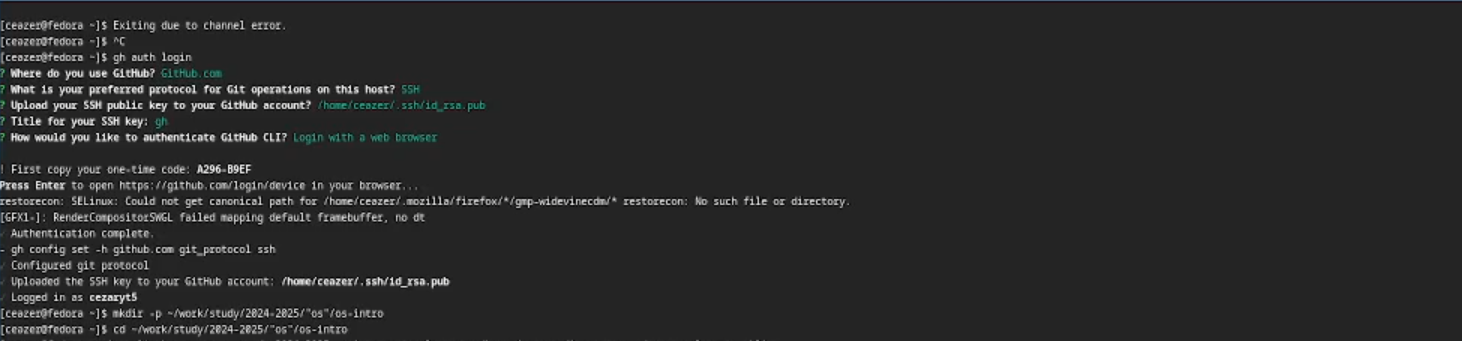
\includegraphics[width=0.9\textwidth,height=\textheight]{./image/gh.png}
\end{column}
\end{columns}
\end{block}

\begin{block}{3.3 Создание репозитория}
\phantomsection\label{ux441ux43eux437ux434ux430ux43dux438ux435-ux440ux435ux43fux43eux437ux438ux442ux43eux440ux438ux44f}
\begin{columns}[c]
\begin{column}{0.6\textwidth}
\begin{itemize}[<+->]
\tightlist
\item
  Создан репозиторий на основе шаблона
\item
  Настроен для хранения всех лабораторных работ
\item
  Готов к работе с Git
\end{itemize}
\end{column}

\begin{column}{0.4\textwidth}
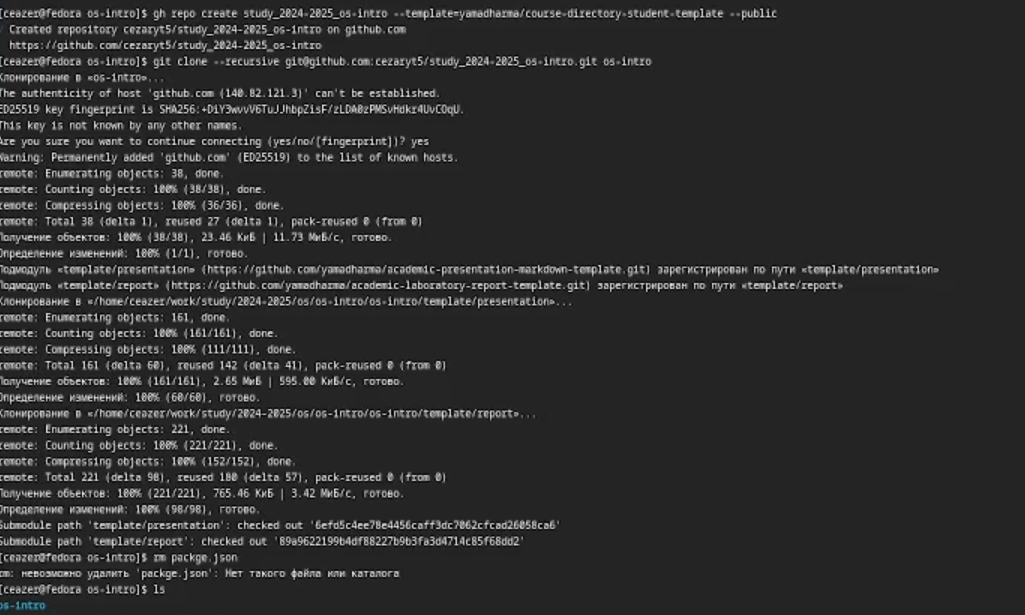
\includegraphics[width=0.9\textwidth,height=\textheight]{./image/repo.png}
\end{column}
\end{columns}
\end{block}

\begin{block}{3.4 Настройка SSH ключей}
\phantomsection\label{ux43dux430ux441ux442ux440ux43eux439ux43aux430-ssh-ux43aux43bux44eux447ux435ux439}
\begin{columns}[c]
\begin{column}{0.6\textwidth}
\textbf{Команды для генерации SSH ключей:}

\begin{Shaded}
\begin{Highlighting}[]
\FunctionTok{ssh{-}keygen} \AttributeTok{{-}t}\NormalTok{ ed25519 }\AttributeTok{{-}C} \StringTok{"mohamed.musa@student.rudn.ru"}
\BuiltInTok{eval} \StringTok{"}\VariableTok{$(}\FunctionTok{ssh{-}agent} \AttributeTok{{-}s}\VariableTok{)}\StringTok{"}
\FunctionTok{ssh{-}add}\NormalTok{ \textasciitilde{}/.ssh/id\_ed25519}
\FunctionTok{cat}\NormalTok{ \textasciitilde{}/.ssh/id\_ed25519.pub}
\end{Highlighting}
\end{Shaded}
\end{column}

\begin{column}{0.4\textwidth}
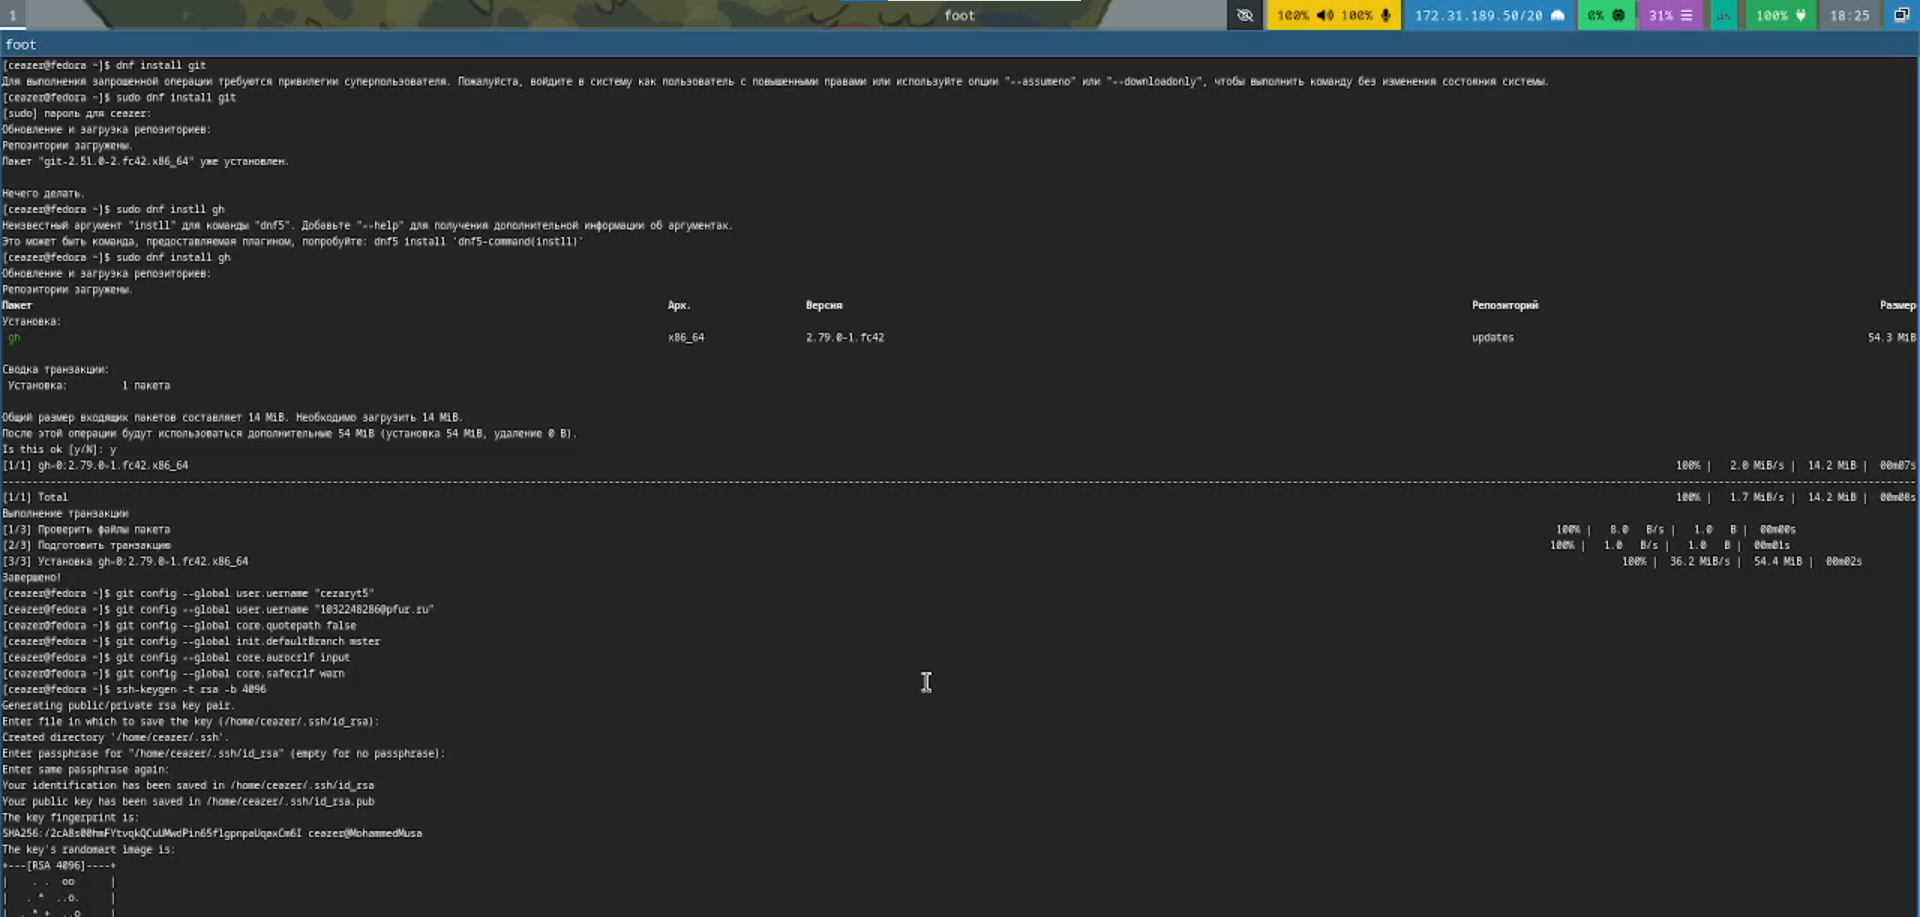
\includegraphics[width=0.9\textwidth,height=\textheight]{./image/ssh.png}
\end{column}
\end{columns}
\end{block}

\begin{block}{3.5 Настройка GPG ключей}
\phantomsection\label{ux43dux430ux441ux442ux440ux43eux439ux43aux430-gpg-ux43aux43bux44eux447ux435ux439}
\begin{columns}[c]
\begin{column}{0.6\textwidth}
\textbf{Команды для генерации GPG ключей:}

\begin{Shaded}
\begin{Highlighting}[]
\ExtensionTok{gpg} \AttributeTok{{-}{-}full{-}generate{-}key}
\ExtensionTok{gpg} \AttributeTok{{-}{-}list{-}secret{-}keys} \AttributeTok{{-}{-}keyid{-}format}\NormalTok{ LONG}
\FunctionTok{git}\NormalTok{ config }\AttributeTok{{-}{-}global}\NormalTok{ user.signingkey }\OperatorTok{\textless{}}\NormalTok{KEY\_ID}\OperatorTok{\textgreater{}}
\FunctionTok{git}\NormalTok{ config }\AttributeTok{{-}{-}global}\NormalTok{ commit.gpgsign true}
\end{Highlighting}
\end{Shaded}
\end{column}

\begin{column}{0.4\textwidth}
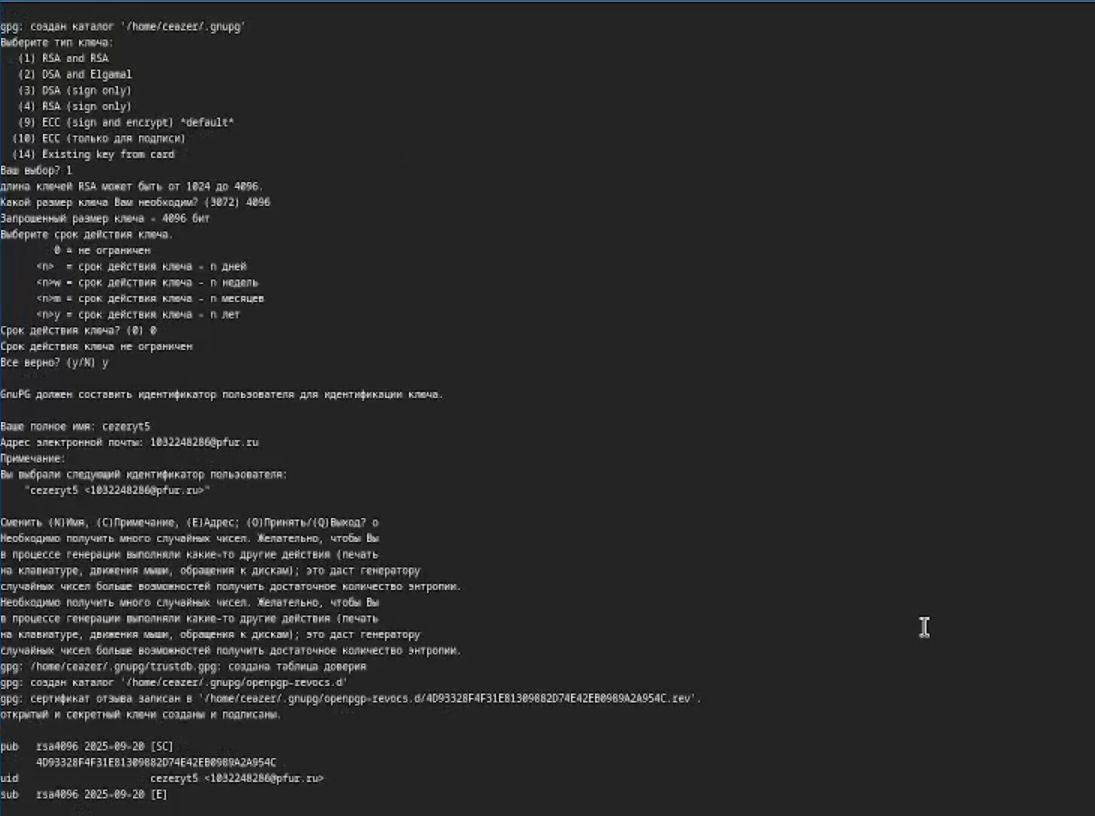
\includegraphics[width=0.9\textwidth,height=\textheight]{./image/gpg.png}
\end{column}
\end{columns}
\end{block}

\begin{block}{3.6 Подготовка структуры}
\phantomsection\label{ux43fux43eux434ux433ux43eux442ux43eux432ux43aux430-ux441ux442ux440ux443ux43aux442ux443ux440ux44b}
\begin{columns}[c]
\begin{column}{0.6\textwidth}
\textbf{Команда сборки проекта:}

\begin{Shaded}
\begin{Highlighting}[]
\FunctionTok{make}
\end{Highlighting}
\end{Shaded}

Подготовка рабочей структуры согласно шаблону.
\end{column}

\begin{column}{0.4\textwidth}
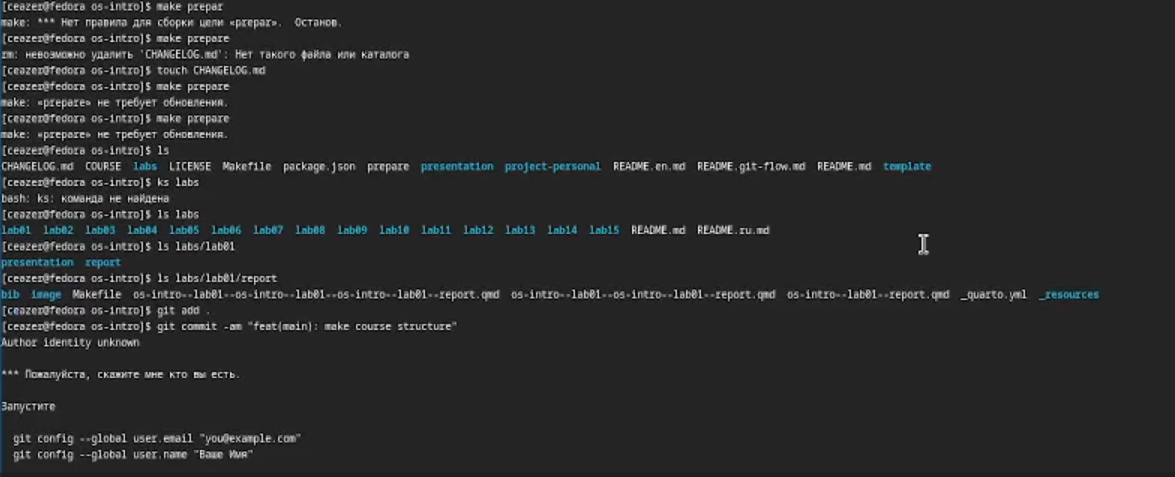
\includegraphics[width=0.9\textwidth,height=\textheight]{./image/make.png}
\end{column}
\end{columns}
\end{block}

\begin{block}{3.7 Глобальные команды Git}
\phantomsection\label{ux433ux43bux43eux431ux430ux43bux44cux43dux44bux435-ux43aux43eux43cux430ux43dux434ux44b-git}
\begin{columns}[c]
\begin{column}{0.6\textwidth}
\textbf{Настройка глобальных параметров:}

\begin{Shaded}
\begin{Highlighting}[]
\FunctionTok{git}\NormalTok{ config }\AttributeTok{{-}{-}global}\NormalTok{ user.name }\StringTok{"Mohamed Musa"}
\FunctionTok{git}\NormalTok{ config }\AttributeTok{{-}{-}global}\NormalTok{ user.email }\StringTok{"mohamed.musa@student.rudn.ru"}
\FunctionTok{ssh} \AttributeTok{{-}T}\NormalTok{ git@github.com}
\end{Highlighting}
\end{Shaded}
\end{column}

\begin{column}{0.4\textwidth}
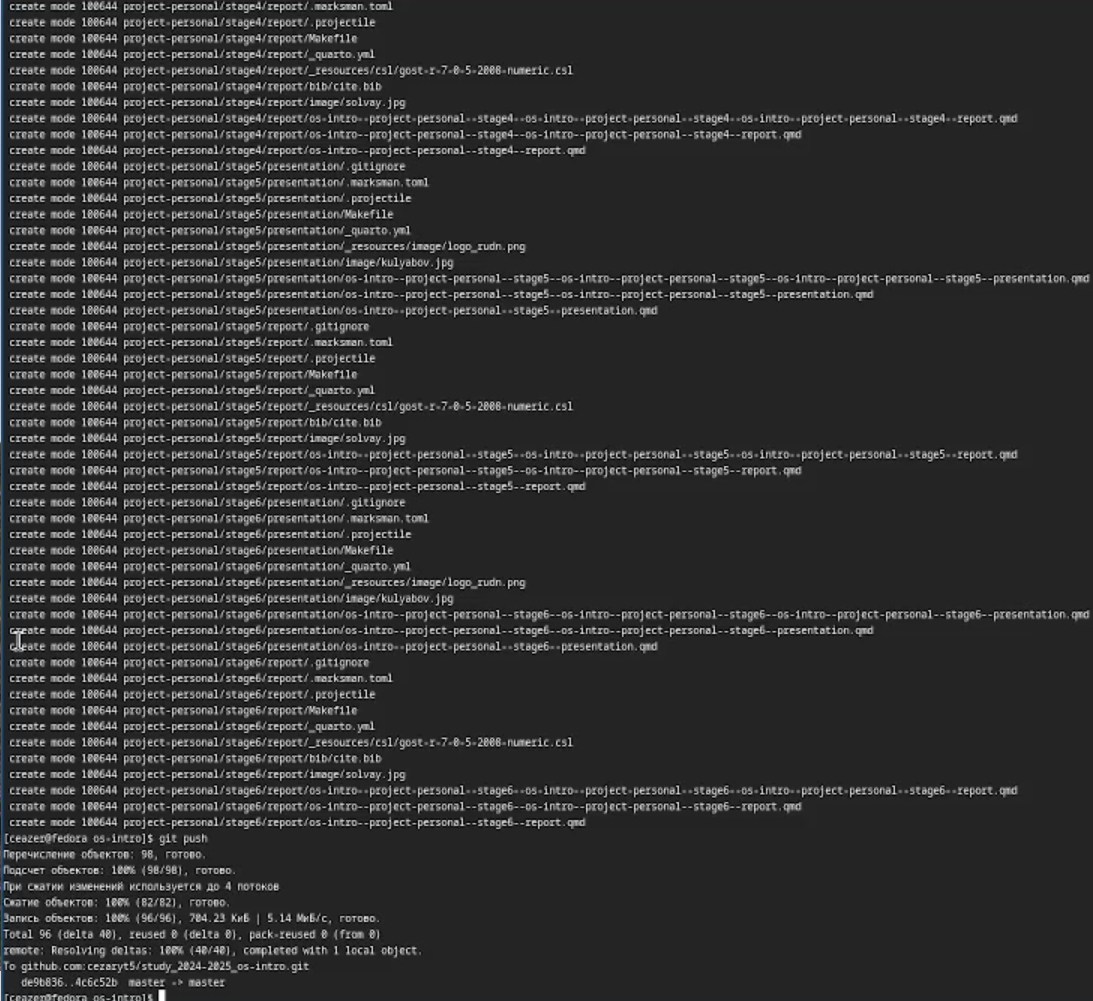
\includegraphics[width=0.9\textwidth,height=\textheight]{./image/push.png}
\end{column}
\end{columns}
\end{block}

\begin{block}{3.8 Отправка изменений}
\phantomsection\label{ux43eux442ux43fux440ux430ux432ux43aux430-ux438ux437ux43cux435ux43dux435ux43dux438ux439}
\begin{columns}[c]
\begin{column}{0.6\textwidth}
\textbf{Операции с репозиторием:}

\begin{Shaded}
\begin{Highlighting}[]
\FunctionTok{git}\NormalTok{ add .}
\FunctionTok{git}\NormalTok{ commit }\AttributeTok{{-}S} \AttributeTok{{-}m} \StringTok{"feat: initial setup with lab template"}
\FunctionTok{git}\NormalTok{ push }\AttributeTok{{-}u}\NormalTok{ origin main}
\end{Highlighting}
\end{Shaded}

Все изменения успешно отправлены в удаленный репозиторий.
\end{column}

\begin{column}{0.4\textwidth}
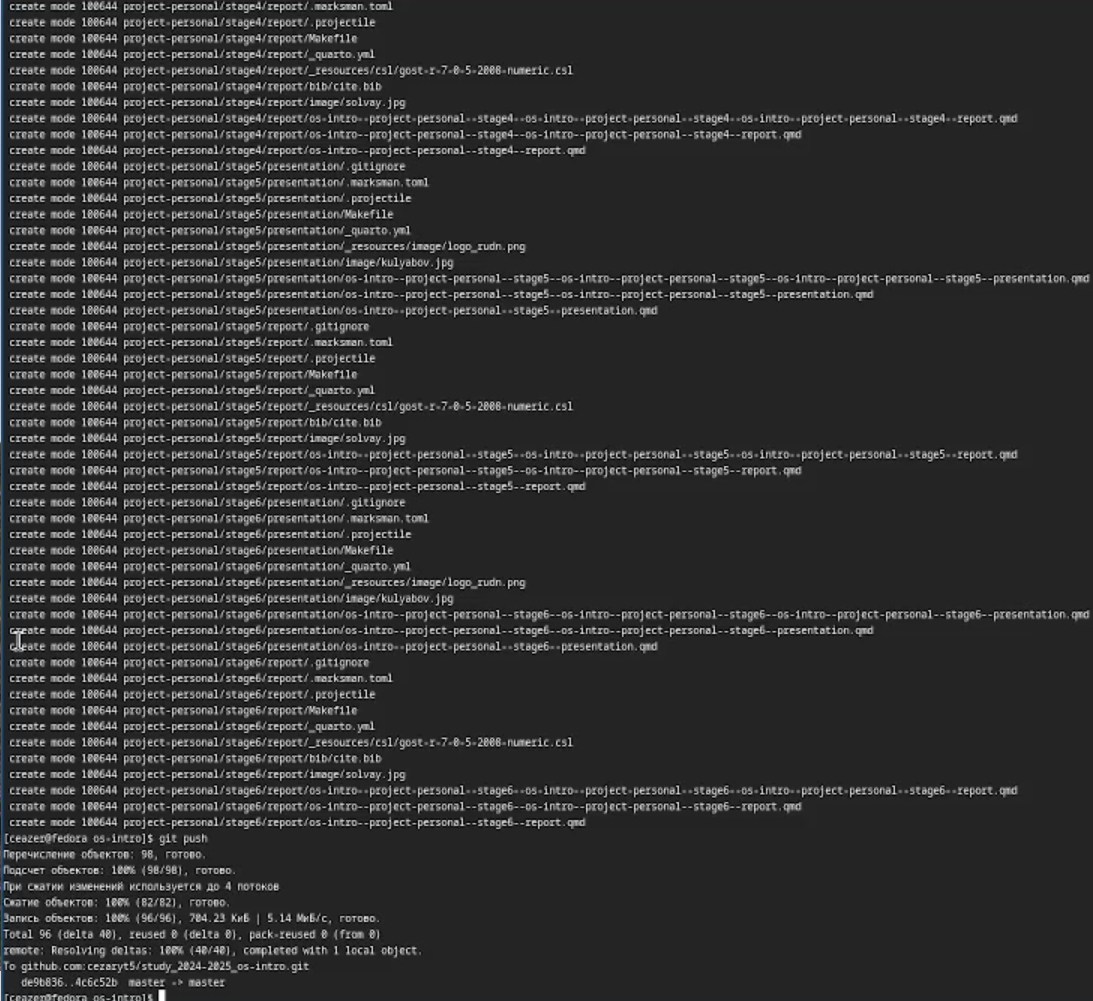
\includegraphics[width=0.9\textwidth,height=\textheight]{./image/push.png}
\end{column}
\end{columns}
\end{block}
\end{frame}

\begin{frame}{4. Выводы}
\phantomsection\label{ux432ux44bux432ux43eux434ux44b}
\begin{block}{4.1 Достигнутые результаты}
\phantomsection\label{ux434ux43eux441ux442ux438ux433ux43dux443ux442ux44bux435-ux440ux435ux437ux443ux43bux44cux442ux430ux442ux44b}
✅ Настроен Git и создан GitHub аккаунт ✅ Созданы SSH ключи для
безопасного подключения ✅ Настроены GPG ключи для подписывания коммитов
✅ Создан и настроен репозиторий для лабораторных работ ✅ Освоены
основные команды Git (add, commit, push, pull) ✅ Выполнены операции с
ветками и слияние
\end{block}

\begin{block}{4.2 Полученные навыки}
\phantomsection\label{ux43fux43eux43bux443ux447ux435ux43dux43dux44bux435-ux43dux430ux432ux44bux43aux438}
\begin{itemize}[<+->]
\tightlist
\item
  Работа с современными инструментами разработки
\item
  Принципы распределенной разработки
\item
  Безопасная аутентификация
\item
  Командная работа над проектами
\end{itemize}
\end{block}
\end{frame}

\begin{frame}{5. Список литературы}
\phantomsection\label{ux441ux43fux438ux441ux43eux43a-ux43bux438ux442ux435ux440ux430ux442ux443ux440ux44b}
\phantomsection\label{refs}
\begin{CSLReferences}{0}{1}
\begin{itemize}[<+->]
\tightlist
\item
  Git Documentation: \url{https://git-scm.com/doc}
\item
  GitHub Guides: \url{https://guides.github.com/}
\item
  SSH Keys Setup:
  \url{https://docs.github.com/en/authentication/connecting-to-github-with-ssh}
\item
  GPG Keys Setup:
  \url{https://docs.github.com/en/authentication/managing-commit-signature-verification}
\item
  Pro Git Book: \url{https://git-scm.com/book/ru/v2}
\end{itemize}

\end{CSLReferences}
\end{frame}



\end{document}
